\documentclass[convert={density=300,size=1080x800,outext=.png}]{standalone}
\usepackage{tkz-graph}
\usetikzlibrary{arrows,positioning,shapes,shapes.multipart,patterns,mindmap,shadows}
\usepackage{xcolor}
\usepackage{helvet}
\renewcommand{\familydefault}{\sfdefault}


\begin{document}

\footnotesize
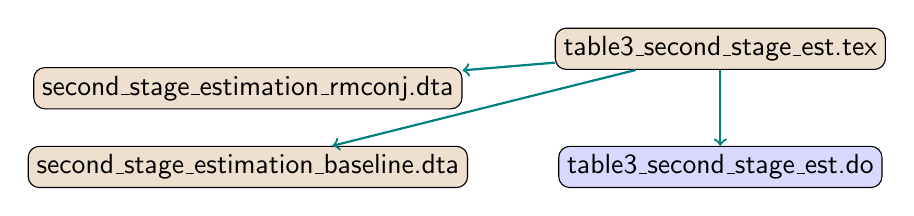
\begin{tikzpicture}[every node/.style={
    rectangle,
    rounded corners,
    inner sep=3pt,
    draw,
    fill=brown!25
}]



    \node (second_stage_estimation_baseline_dta) [shift={(9, -4)}]
    {
        second\_stage\_estimation\_baseline.dta
    };

    \node (second_stage_estimation_rmconj_dta) [shift={(9, -3)}]
    {
        second\_stage\_estimation\_rmconj.dta
    };





    \node (table3_second_stage_est_tex) [shift={(15, -2.5)}]
    {
        table3\_second\_stage\_est.tex
    };

    \node (table3_second_stage_est_do) [fill=blue!15, shift={(15, -4)}]
    {
        table3\_second\_stage\_est.do
    };


    \draw[->, teal, thick] (table3_second_stage_est_tex) to (table3_second_stage_est_do);
    \draw[->, teal, thick] (table3_second_stage_est_tex) to (second_stage_estimation_baseline_dta);
    \draw[->, teal, thick] (table3_second_stage_est_tex) to (second_stage_estimation_rmconj_dta);


\end{tikzpicture}

\end{document}

